\chapter{Conclusions and Future Work}

\epigraph{``...and the credits rave as the critics roll.''}
{{\sl Mike Vennart, Silent/Transparent}}

I began this thesis with the statement that accreting systems
and their associated outflows are astrophysically important. However, I also
demonstrated that much of the diverse phenomenology associated with such systems, as well
as the underlying {\em physics}, is not well understood.  
Having attempted to address some of the issues raised in the 
introductory chapters, I will provide some concluding remarks. 
First, I will summarise my findings, before 
commenting on how future research can help unveil the true nature of 
accretion discs and their winds.

A large portion of this PhD has been spent maintaining,
testing and developing the MCRT and ionization code, \py. The first 
step in this project was to understand the macro-atom scheme
developed by \cite{lucy2002,lucy2003}, and its specific integration
into \py. I described the scheme and the operation of \py\ in detail
in chapter 3, partly in the hope that it will prove a useful document
for future efforts involving this powerful, but complex, piece of software.
The latter parts of the same chapter focused on the series of tests
I conducted to robustly verify that the code worked as expected and 
could reproduce the expected analytical and computational results in certain
physical limits. Near the start of the project many of these tests
would fail, either because \py\ did not possess the relevant atomic data,
or because the necessary integration between the macro-atom and simple-atom
portions of the code was not yet in place. Thus, while time consuming,
progressing to the point where all the tests shown in chapter 3 could be
passed was an important milestone, and enabled the techniques in question
to be applied to astrophysical problems with confidence.

The first of these astrophysical problems involved CVs, and in particular
those accreting at a relatively high rate, such as DNe or NLs. Having 
improved the radiative transfer techniques from previous CV modelling efforts
involving \py\ \citep[LK02, ][]{noebauer}, it was now possible to see
if the outflows that are responsible for the P-Cygni profiles seen
in UV resonance lines could also affect the {\em optical} line and continuum
emission. The results are unambiguous. By simply taking the SV93/LK02
models -- designed to reproduce the UV spectra of high-state CVs --
and `turning on' the improved radiative transfer mode, the wind
has a significant effect on the optical spectrum, producing strong
\ha, \heiiopt\ and \heiioptnew\ lines, among others, at high inclinations.

I then conducted a small parameter search over just two kinematic parameters, 
to see if a model could produce {\em all} of the optical H and He lines observed 
in high-state CVs. Synthetic spectra from a model 
with a more slowly accelerating outflow show 
the full sequence of H and He recombination lines, with 
the observed trend from strong emission at high inclination to weaker lines
at low inclination. Furthermore, the dense outflow now produces strong Balmer
recombination emission that is sufficient to `fill in' the Balmer 
absorption edge intrinsic to the disc atmosphere input spectrum. The optically
optimised model is not without issues; the red wing to the \civ\ line
is now overly strong, particularly at high inclinations, and \heii\ emission
is stronger than that observed. Nevertheless, the synthetic spectra exhibit
reasonable verisimilitude with observations of the high inclination NL RW Tri,
and the results indicate that disc winds may have a much broader impact,
especially in wavelength terms, than is traditionally expected. Furthermore,
the large vertical extent of the line emitting region has implications
for techniques that assume planar line emission, such as Doppler tomography 
\citep[e.g.][]{marsh1988} and eclipse mapping \citep[e.g.][]{horne1994}.

In chapter 5, I applied similar techniques to the question of quasar 
unification, but with one additional adaptation. In order to simultaneously
increase the emission measure of the wind, as well as moderate the ionization
state in the presence of strong X-rays, I incorporated a simple treatment of clumping 
into \py. The technique -- known as microclumping -- is prevalent 
in the stellar wind community, but this was the first time it had been
applied to quasar winds in this context. Although the motivation for including
clumping was in some sense empirical, in that H13 could not produce a 
model with strong \civ\ BALs without severely limiting the X-ray luminosity, 
the validity of this approach is strengthened by the theoretical and observational
evidence for clumping in line-driven hot star winds 
(see sections~\ref{sec:clumpy_stellar} and \ref{sec:line_driving}).

Once again, I conducted a parameter search, this time in 5 dimensions. 
A broad family of models produce strong UV emission lines at low inclinations
and UV BALs at high inclinations. 
Thus, the first success of the clumpy quasar wind model is that,
for clumping factors comparable to those required 
in stellar wind modelling \citep{hamann2008}, the ionization
state of the wind matches well with observations despite the presence
of strong X-ray radiation. Indeed, the X-ray properties of the model now 
agree well with observed non-BAL and BAL quasar values for $L_X$, suggesting
that the partially self-shielding BAL outflow itself might be responsible 
for the observed X-ray weakness of BAL quasars. Perhaps the most
compelling attribute of the wind model is that it naturally reproduces
the broad range of ionization states observed in AGN, such that the wind 
emission has very similar characteristics to the observed BLR spectrum 
(see, e.g., Fig.~\ref{fig:sed}). The primary limitation of the fiducial
quasar model is a geometric one; it is not possible to produce comparable
line EWs at low inclination to those at high inclination, due to the
foreshortened, limb-darkened, and absorbed disc emission. Thus, even 
if the low inclination line emission could be matched to the observed quasar EWs,
the model would then over-predict the line emission emerging at high inclination
`BALQSO-like' angles. This suggests an issue with an equatorial unification model,
and provides the motivation for exploring the observational
characteristics of emission lines in BAL and non-BAL quasars.

The final project in this PhD saw a switch in philosophy, as, informed
by the radiative transfer modelling, I turned to observations and in particular
the invaluable dataset that is the {\sl Sloan Digital Sky Survey}. 
The aim of this exercise was to more quantitatively assess the apparent
similarity in emission line properties in BAL and non-BAL quasars. I first
reproduced the results of \cite{risaliti2011} using the updated dataset 
by fitting the distribution of the EW of the \oiiifull\ emission line 
with a simple geometric model, in which an intrinsic Gaussian distribution
was convolved with the expected angular distribution of quasars expected in a 
flux-limited sample. I then constructed a toy model for geometric unification,
and showed that predictions from the simplest quasar wind models -- 
those where an equatorial outflow rises from a geometrically thin, 
optically thick accretion disc -- are not consistent with the observed 
EW distributions of quasar emission lines. The results also suggest that
obscuration is not the key driver of the \ewo\ distribution -- albeit
under the assumption that LoBAL
quasars are drawn from the same population as non-BAL quasars.

The overall conclusions of this final study are striking, and extend 
beyond just constraining BAL outflow parameters. 
They suggest a few possible scenarios; perhaps quasar discs are much
more isotropic than one might expect. If this is the case, how is it
reconciled with accretion disc theory? Alternatively, BAL and
non-BAL quasars may be viewed from a similar range of angles, in 
which case their differences in polarisation properties must be 
understood. The final possibility is, of course, that geometric unification
does not explain the incidence of BALs in the UV spectra of quasars.
This final scenario is not a solution to the problem, {\sl per se}. After all, BAL
outflows {\em must} emerge at some range of angles, and this range of 
angles is important to constrain in order to understand the outflow physics.

Perhaps unsurprisingly, the work presented in this thesis has raised 
many questions, some of which are fundamental to our understanding of CVs, 
quasars and accreting systems genera lly. I
will therefore devote some time to discussing what I believe are 
natural next steps in furthering our understanding of accretion
and outflow on all scales.

\section{Suggestions for Future Work}

\subsection{CVs as Accretion and Outflow Laboratories}

CVs are the closest and best understood laboratories for
our understanding of accretion physics. In particular, the NL
variables make excellent testbeds for the $\alpha$-disc model,
as they are one of the few accreting systems known to
lie in a relatively constant accretion rate state -- fulfilling 
an explicit assumption of the SS73 prescription. I suggest
that two observational programs relating to NLs are pursued.
The first is to take broadband, simultaneous spectroscopy of a number
of NL variables. This will allow the impact of winds on the spectrum
to be assessed more carefully as modelling of the entire wavelength
range can be undertaken, possibly including fits to the observed spectrum.
It will also allow the broadband SED to be fitted with confidence,
and inferences made about the temperature profile of the disc. 
Our team recently submitted an HST proposal (PI: Long) with this brief.
The second is to take measurements of the depth of the Balmer jump
in a relatively large sample of NLs, either through narrow band spectroscopy
or two-band photometry. Together with inclination measurements the predictions
of disc and outflow models can be tested directly by exploring how the depth
of the Balmer absorption edge varies with viewing angle and accretion rate.

\subsection{Improving the Treatment of Clumping}

One of the limitations of the work presented in chapter 5 is that the
treatment of clumping is fairly simple, and does not adequately capture the
physics of potential dense substructures in AGN outflows. 
Indeed, it is considered a `first step' towards
accurately including clumpiness in \py. So, what is the next step? One fairly 
simple way of including some degree of porosity in the treatment would 
be to relax the assumption that the Sobolev length is larger than the
clump size. The Sobolev optical depth can then be calculated either
or in or out of a clump, based on a random number choice proportional
to the clump filling factor. This would mean that there is a chance 
that photons will not interact with clumps, possibly leading to
the non-black saturation that is observed in BAL troughs 
\citep[][see also section~\ref{sec:balqso_angles}]{arav1999b,arav1999a}.
More generally, an approach similar to macroclumping, as 
used in stellar wind modelling \citep[e.g.][]{hamann2008,surlan2012},
would allow the inclusion of porosity.

More complex approaches could also be considered here, 
such as the `two-phase' ideas used in clumpy torus models 
\citep{stalevski2013} and suggested for the BLR 
\citep[e.g.][]{netzer1990, dekool1995, elvis2000}.
However, the general problem here is that, while introducing more freedom into 
the wind model would certainly allow one to fit quasar and CV spectra
more effectively, the question is whether this provides useful physical insight.
This is somewhat open to interpretation, as the filling factors and origins of clumps
in BLR and outflow models are not well constrained. I would therefore suggest that
some of the above techniques are implemented, and experimented with,
but would urge caution with regards to the interpretation of the overall
results. As mentioned in chapter 4, including clumping in the CV modelling
could prove particularly interesting with regards to the optical P-Cygni profiles 
observed in He~\textsc{i} and \ha\ in some CVs. 
Intriguingly, similar profiles were also 
seen during the recent outburst of V404 Cyg \citep{munozdarias2016}.

\subsection{Improving Atomic Models}

Although treating both hydrogen and helium as a macro-atom was
a significant improvement over the previous two-level approaches, 
much can still be done to improve how \py\ deals with atomic processes.
One of the main limitations of the code is the current treatment of
collisions, as discussed in chapter 4. One way to improve the accuracy
of collision strengths between dipole transitions would be to use
experimental data \citep[e.g.][]{gaetz1983}. 
% This will allow for more 
% accurate collision strengths to be calculated.
% Although this is unlikely to change the overall temperature and ionization
% structure of any of the wind models, but could lead to more accurate line 
% ratios when the lines are collisionally excited. This will also lead to 
% more accurate values of line heating and cooling, which is particularly
% important in the CV model where 
I have also recently begun an effort to incorporate macro-atom data for
additional elements. The fundamental aim of this is to
be able to introduce a series of more complex atoms that cannot be modelled 
with the two-level approach, so that, for example, the density-dependent 
phosphorous doublets or semi-forbidden C~\textsc{iii}] 
line could be accurately reproduced in spectra. 
Fig.~\ref{fig:carbon_matom} shows how a carbon macro-atom
has been incorporated into the code and produces reasonable results for moderate
ionization stages, although there are still some ongoing issues.

\begin{figure} 
\centering
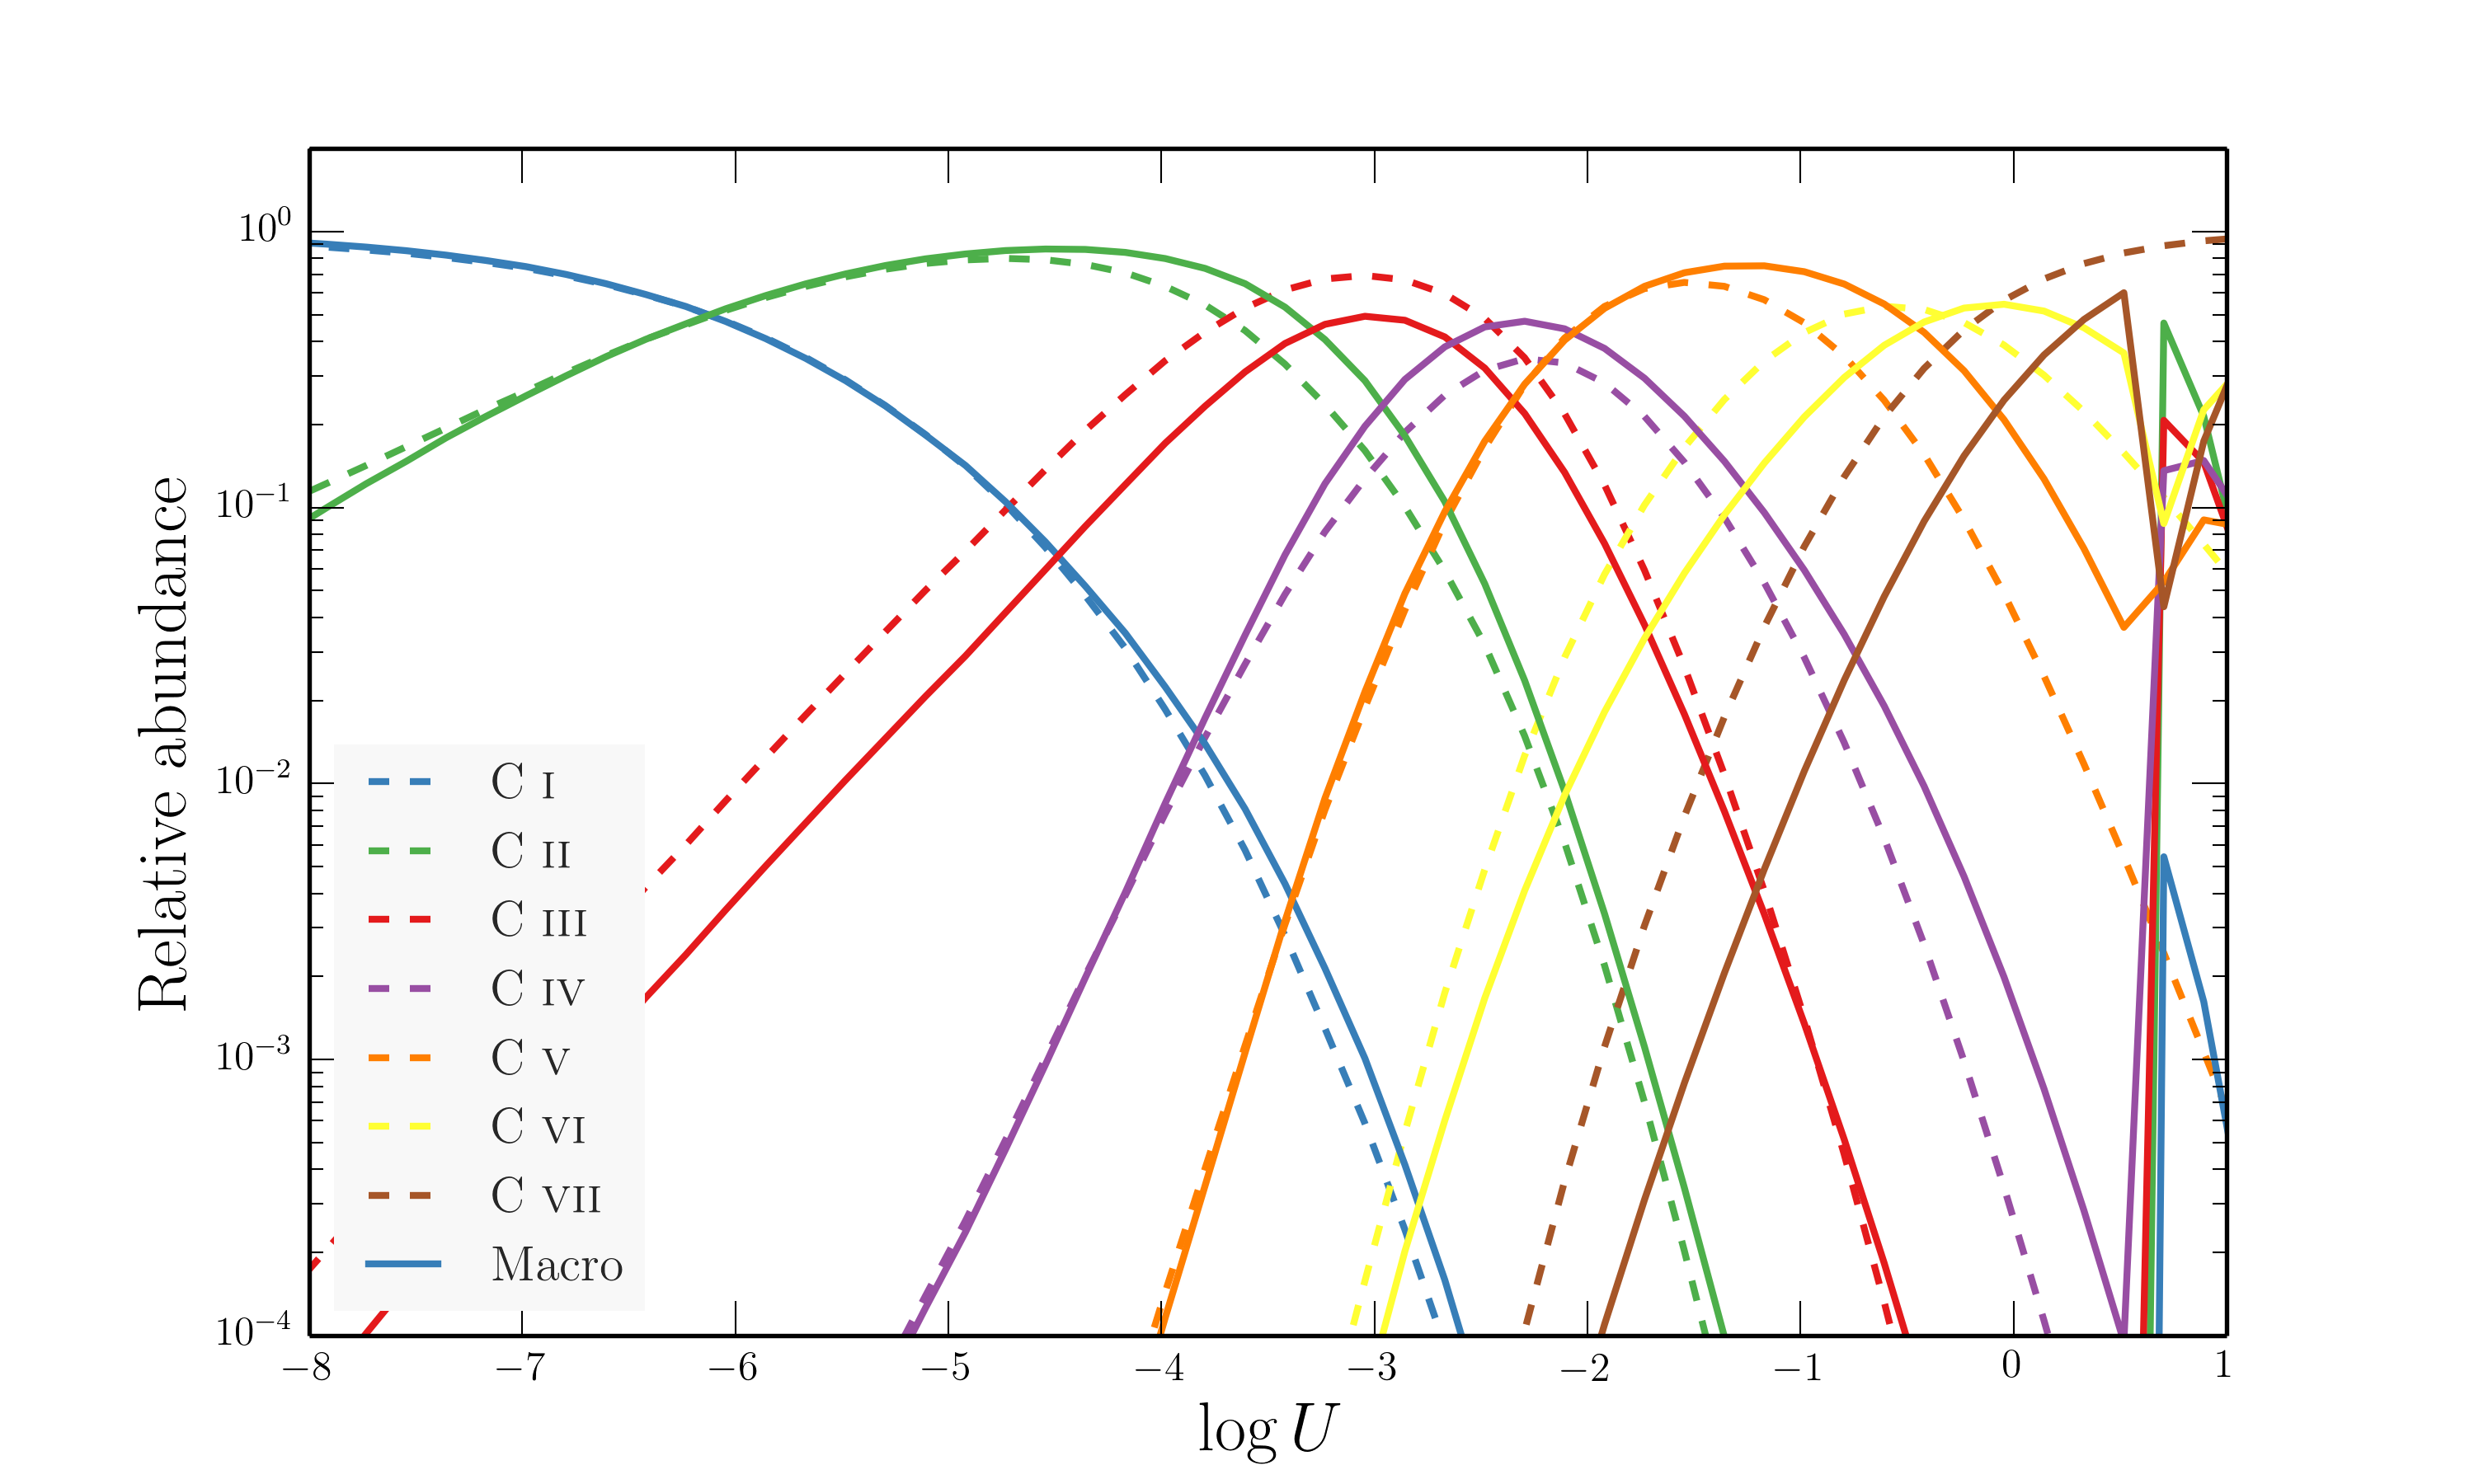
\includegraphics[width=0.8\textwidth]{figures/ewpaper/carbon_matom_ion.png}
\caption
[Ion fractions as a function of ionization parameter when 
Carbon is treated as a simple-atom and macro-atom.]
{
Ion fractions as a function of ionization parameter when 
Carbon is treated as a simple-atom (dotted lines) or macro-atom (solid lines)
Although serious, as yet unsolved, numerical problems appear at 
high ionization parameters, the fundamental machinery for treating
Carbon as a macro-atom is now in place.
}
\label{fig:carbon_matom}
\end{figure} 


\subsection{Using Radiative Transfer to Make Reverberation and Microlensing Predictions}

I described in the introduction how the `accretion disc size problem' poses
a profound challenge to the current best-bet model for the AGN continuum.
I suggest that radiative transfer with \py\ is used to predict the 
reverberation and microlensing signatures from wind models for AGN and quasars. 
The former has already been started by Sam Mangham as part of a PhD
project, and an example transfer function from the fiducial quasar wind model
is shown in Fig.~\ref{fig:halpha_transfer}. With the machinery now in place,
the continuum lags from such a model can be computed and compared to observations.
This will particularly useful if it is possible to produce a reasonable wind
model for NGC 5548, as comparisons can then be made to the long-term monitoring
campaigns \citep[e.g.][]{edelson2015} to assess if a wind can produce the observed 
lags, including the excess lag in the Balmer continuum that can now be modelled 
in \py\ with the macro-atom scheme. MCRT can also be used to predict 
the microlensing signatures from wind and BLR models. If \py\ is modified to produce
spatially-resolved images, binned in frequency space, as a function of viewing 
angle, then these can be directly fed into the microlensing analysis. This will
allow for an independent test of the microlensing models themselves, as well as
making predictions for the sizes associated with line and continuum emission from
outflows. 

\begin{figure} 
\centering
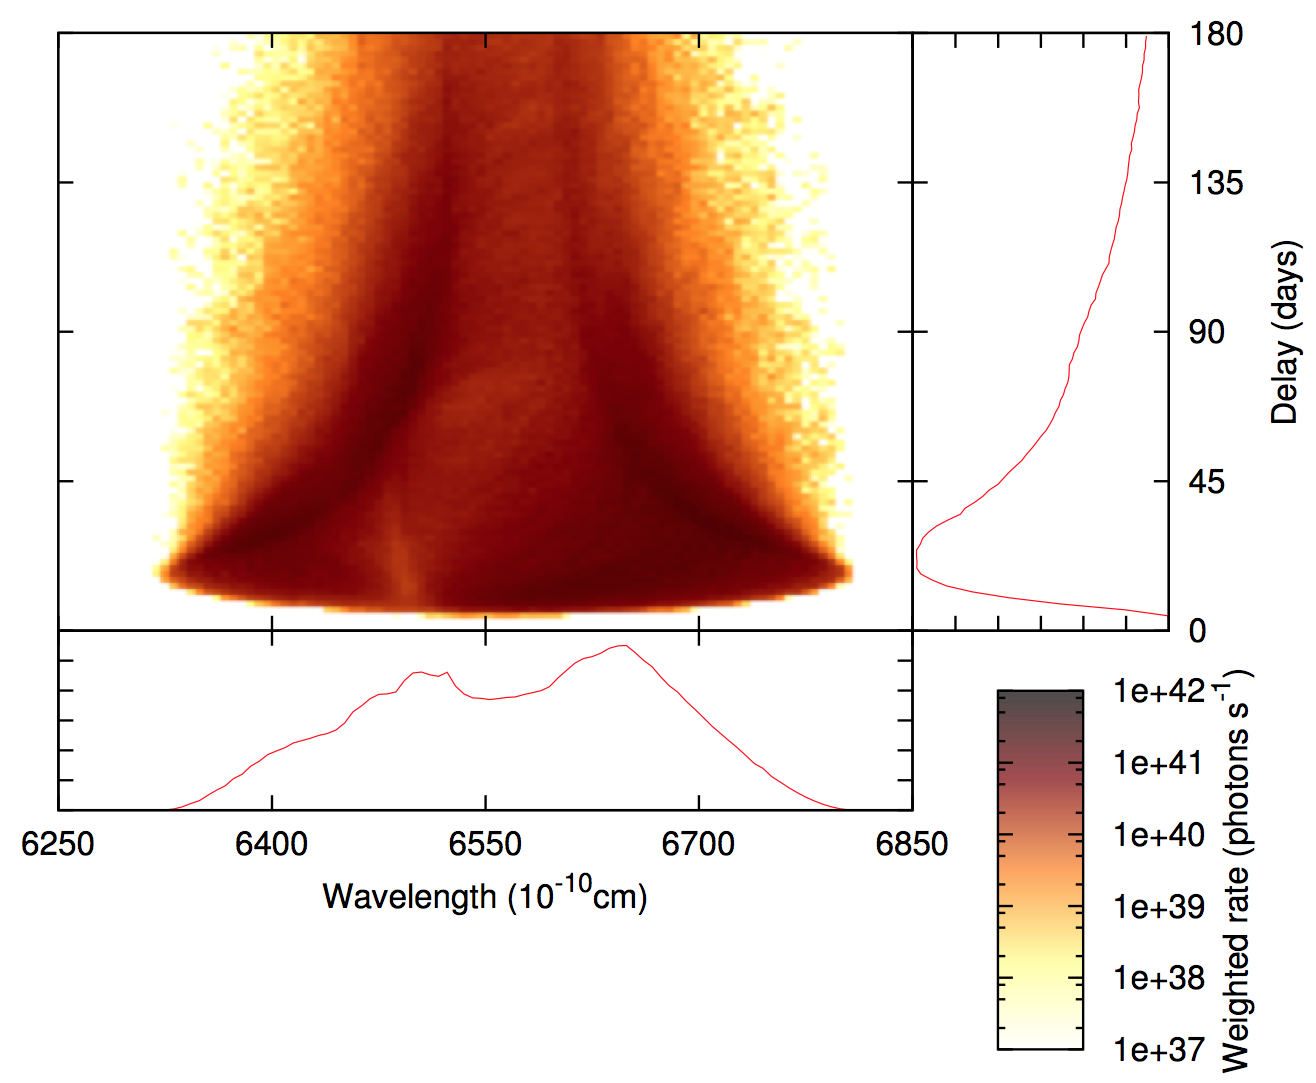
\includegraphics[width=0.7\textwidth]{figures/ewpaper/halpha_transfer.png}
\caption
[Velocity-resolved transfer function for \ha\ 
from the fiducial quasar model.]
{
{\sl Credit: Sam Mangham.}
Velocity-resolved transfer function for \ha\ 
from the fiducial quasar model presented in
chapter 5. The transfer function is for a viewing angle of 
$40^\circ$. 
}
\label{fig:halpha_transfer}
\end{figure} 

\subsection{Placing BAL Quasars on the Eigenvector 1 Parameter Space}

In chapter 6 we saw how LoBAL quasars are not specifically clustered
in one region of parameter space on the so-called `Eigenvector 1'
diagram. Under the interpretation of \cite{shenho2014}, this implies that
no preferred inclination, although there is a suggestion
of an overdensity towards the upper right quadrant of the parameter space 
(see Fig.~\ref{fig:bal_ev1_bins}). Ideally, I would have been able to
also plot the HiBAL quasars in this space, particularly as LoBAL quasars
may not be drawn from the same population as normal type 1 quasars 
\citep[e.g.][]{urrutia2009,dai2012}. I would thus advocate targeting an
SDSS-selected sample of HiBAL quasars, in the redshift range $1.45<z<2.28$,
with near infra-red telescopes in order 
to obtain rest-frame optical spectroscopy covering
\hb, \oiiifull\ and the broad Fe~\textsc{ii} emission underlying \hb. This
would allow HiBAL quasars to be placed successfully in EV1 space, and in the 
process provide \ewo\ measurements. The fitting of the \ewo\ distribution
I carried out in chapter 6 for LoBALs could then be repeated on this HiBAL sample.

\section{Closing Remarks}

Disc winds are ubiquitous in accreting systems and have a 
profound connection with the accretion process. I have demonstrated,
through state-of-the-art MCRT simulations, that disc winds extend their
influence beyond the blue-shifted BALs and P-Cygni profiles traditionally
associated with outflow. They may produce the optical line and continuum emission
in CVs, possibly even dominating the observed spectrum. Simple clumpy biconical
wind models also naturally exhibit the range of ionization states
and emission lines seen in type 1 AGN and quasars, and once again
may significantly alter the continuum shape. Regardless of their true
impact, the influence of disc winds on the spectra of accreting systems
must be understood, and the outflow covering factors and opening angles 
accurately estimated, for three main reasons. First, so that the feedback 
efficiency of BAL outflows, and mass-loss rates in CVs,
can be calculated. Second, so that the true intrinsic continuum can be unveiled, and 
the viability of the current `best-bet' accretion disc models can be assessed. 
Third, so that the orientations of AGN and quasars can be properly constrained,
allowing us to unify their diverse phenomenology. 
These questions are still unanswered, but I hope that in this thesis I have
demonstrated that {\em disc winds matter}, and are fundamental
to our understanding of accreting compact objects.